\subsection{Optimisation et amélioration du nouveau modèle}
%TODO passer add to cat dans cette partie ?

%opti 1
	%addcat
	%reprise train
	%batch
%pb mémoire (beaucoup d'opti perf nécessite d'augmenter la taille des params/modules/tenseurs...) & tps (la plupart des otpis perfs augmentent le tps de calcul nécessaire, et de base le modele naif est trop lent)
%pb memoire réglé, tentative infructueuse d'améliorer les perfs avec améliorations préparées en parallèle
	%+ params
	%lbl
% ccl plus pb mémoire & tps, opti z'oignons (XD) même, 5 min c'est balèze

Une fois le prototype fonctionnel, il à fallu améliorer les performances.
Par performances, nous entendons principalement le temps nécessaire pour que la qualité prédictive du modèle dépasse un certain seuil.

Pour améliorer ce temps de calcul, il est possible de travailler sur deux dimensions~:
\begin{itemize}
	\item la \textbf{quantité de données} traitées en un laps de temps~; c'est une \textbf{stratégie quantitative}~;
	\item la \textbf{qualité} de l'apprentissage pour une quantité fixée de données~; c'est une \textbf{stratégie qualitative}.
\end{itemize}

Ainsi, plusieurs options sont possible~:
\begin{itemize}
	\item optimiser les algorithmes et le modèle pour réduire le temps nécessaire pour traiter les données~;
	\item améliorer le modèle en réglant les paramètres (comme la fréquence de transmission) ou en implémentant de nouvelles mécaniques~;
\end{itemize}
\hspace{1em}

Les deux stratégies ont été utilisées. Il faut noter que certaines améliorations qualitatives ont un impact quantitatif négatif.

Principalement, le travail effectué pendant cette partie du projet est un travail de débogage et d'analyse et d'optimisation, avec peu d'implémentation de nouvelles mécaniques dans le \gls{model}.

\subsubsection[Agrégation des sorties des couches]{Agrégation des sorties des couches~: d'une stratégie additive à une concaténation}
La première optimisation à été de changer la façon de regrouper les informations de toues les \og échelles\fg{} avant de les transmettre au module produisant la distribution de probabilité.

Initialement, les sorties de toues les \og échelles\fg{} étaient sommées. Cela permettait de maintenir des \glspl{tensor} de dimensions uniformes quel que soit le nombre d'\og échelle\fg{} (\autoref{fig:add}).

Après discussion avec notre maître de stage, la stratégie d'agrégation à été changé en une concaténation des sorties (\autoref{fig:cat}).

\begin{figure}[ht]
	\begin{subfigure}{0.45\textwidth}
		\centering
		\scalebox{1}{\def\layersep{5em}
\begin{tikzpicture}[shorten >=1pt,->,draw=black, node distance=\layersep]
\tikzstyle{every pin edge}=[<-,shorten <=1pt]
\tikzstyle{block}=[minimum size=2em];
\tikzstyle{value}=[rectangle, fill=green!50,block];
\tikzstyle{operation}=[block, circle,inner sep=0pt, fill=red!50];
\tikzstyle{nonlinearity}=[rectangle,block, fill=blue!50];
\tikzstyle{annot} = [text width=6em, text centered]

% Draw the input layer nodes
\foreach \name / \y in {1,...,3}
% This is the same as writing \foreach \name / \y in {1/1,2/2,3/3,4/4}
\node[value, label={[]north:{\'{E}chelle \y}}] (I-\name) at (0,-2*\y) {\y};
\node[value, label={[]north:{\'{E}chelle 4}}, opacity=.5] (I-4) at (0,-8) {4};

% Draw the output layer node
\node[operation, right of=I-2] (ope) {{\Large +}};
\node[value, right of=ope, label={[]north:$1+2+3+4$}](cat){};
% Draw the output layer node
%\node[nonlinearity, right of=cat] (lin) {Lin};
%\node[annot, right of=lin, text width=7em,xshift=2em ] (out) {Distribution de probabilit\'{e}s};

% Connect every node in the input layer with every node in the
% hidden layer.
\foreach \source in {1,...,3}
\path (I-\source.east) edge (ope);
\path (I-4.east) edge[dashed, opacity=.5] (ope);
\path (ope) edge (cat);
%\path (cat) edge (lin);
%\path (lin) edge (out);
\end{tikzpicture}}
		\caption[Stratégie d'agrégation additive]{Stratégie d'agrégation additive.\vspace{2em}}\label{fig:add}
	\end{subfigure}
	\begin{subfigure}{0.45\textwidth}
		\centering
		\scalebox{1}{\def\layersep{5em}
\begin{tikzpicture}[shorten >=1pt,->,draw=black, node distance=\layersep]
    \tikzstyle{every pin edge}=[<-,shorten <=1pt]
    \tikzstyle{block}=[minimum size=2em];
    \tikzstyle{value}=[rectangle, fill=green!50,block];
    \tikzstyle{operation}=[block, circle,inner sep=0pt, fill=red!50];
    \tikzstyle{nonlinearity}=[rectangle,block, fill=blue!50];
    \tikzstyle{annot} = [text width=6em, text centered]

    % Draw the input layer nodes
    \foreach \name / \y in {1,...,3}
    % This is the same as writing \foreach \name / \y in {1/1,2/2,3/3,4/4}
        \node[value, label={[]north:{\'{E}chelle \y}}] (I-\name) at (0,-2*\y) {\y};
	\node[value, label={[]north:{\'{E}chelle 4}}, opacity=.5] (I-4) at (0,-8) {4};

    % Draw the output layer node
    \node[operation, right of=I-2] (ope) {Cat};
    \node[value, right of=ope](cat){2};
    \node[value, above of=cat, node distance=2.1em]{1};
    \node[value, below of=cat, node distance=2.1em](3){3};
    \node[value, below of=3, node distance=2.1em, opacity=.5]{4};
    % Draw the output layer node
    \node[nonlinearity, right of=cat] (lin) {Lin};
	\node[annot, right of=lin, text width=7em,xshift=2em ] (out) {Distribution de probabilit\'{e}s};

    % Connect every node in the input layer with every node in the
    % hidden layer.
    \foreach \source in {1,...,3}
        \path (I-\source.east) edge (ope);
	\path (I-4.east) edge[dashed, opacity=.5] (ope);
	\path (ope) edge (cat);
	\path (cat) edge (lin);
	\path (lin) edge (out);
\end{tikzpicture}}
		\caption[Stratégie d'agrégation par concaténation]{Stratégie d'agrégation par concaténation. Les sorties sont mises côte-à-côte affin de former un nouveau \gls{tensor}.}\label{fig:cat}
	\end{subfigure} 
	\caption{Stratégies d'agrégation}
\end{figure}

La stratégie par concaténation est plus lente en terme de temps de calcul que la stratégie additive, cependant pour le même temps de calcul elle permet d'obtenir de meilleurs résultats (\autoref{fig:addcat}).

Voir l'annexe \ref{subsec:addcat} pour plus de détail sur le choix de la stratégie d'agrégation. 

\begin{figure}[H]
	\centering
	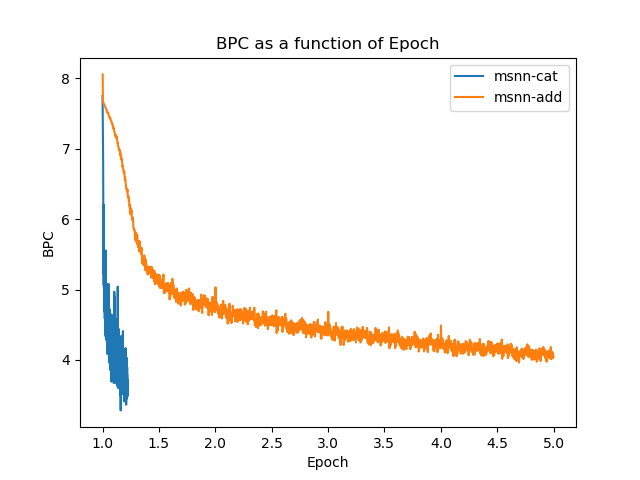
\includegraphics[width=\textwidth]{parts/appendix/reports-gmsnn/docs_esteban-latex/test_reports/comparative-bpc-msnn-det-msnn-cat.png}
	\caption[Performances comparées des stratégies additive et par concaténation]{Performances comparées des stratégies par concaténation (msnn-cat) et additive (msnn-add). Le temps de calcul alloué est identique. Avec la concaténation on entraîne le modèle sur 1/4 des données, avec l'addition on l'entraîne 5 fois sur l'ensemble des données. Avec la concaténation, on obtient une BPC de 3.5, alors qu'on obtient une BPC de 4 avec l'addition.}\label{fig:addcat}
\end{figure} % new

\subsubsection{Sauvegarde, interruption et reprise de l'entraînement}
Une fonctionnalité s'est très vite détachée comme essentielle~: la sauvegarde du \gls{model} et la reprise de l'entraînement.

En effet, avec des entraînements très lents et donc longs, il était nécessaire de pouvoir suspendre l'entraînement affin de répartir le temps de calcul sur plusieurs session de plusieurs heures. De plus, les sauvegardes permettent de conserver le modèle une fois entraîné.

Le système implémenté permet d'effectuer cycliquement des sauvegarde du modèle ainsi que de l'état de l'entraînement, permettant ainsi une reprise en l'état de l'entraînement.

Pour la réalisation du système, le principal obstacle à été le malfonctionnement initial des outils fournis par \gls{pytorch}.
Cela à poussé à la conception d'un système de sauvegarde personnalisé mais malheureusement assez complexe.
Cependant, la mise-à-jour majeure de la librairie qui c'est déroulé à point nommé à résolu le problème, et c'est avec les outils de \gls{pytorch} que le système de sauvegarde à été implémenté.

Voir l'annexe \ref{subsec:save} pour un rapport contenant plus de détail sur le système de sauvegarde. % new
\subsubsection{Tentatives d'optimisations, fuites mémoires et lenteur de l'entraînement}\label{subsec:optimem}

Les optimisations tentées par la suite ont révélé des fuites mémoires et mis en avant une lenteur excessive de l'apprentissage.

Les optimisations en questions ont été mises en suspens le temps de la résolution de ces deux problèmes.
Ces optimisations sont:
\begin{itemize}
	\item l'utilisation de \glspl{batch} simultanés (voir \autoref{subsec:optibatch})~; 
	\item l'augmentation du nombre de \glspl{parameter} du \gls{model} (voir \autoref{subsec:optiparam})~;
\end{itemize}

%\hspace{1em}
\paragraph{Consommation de mémoire et de temps de calcul accrue}
Un effet direct de ces optimisations est l'augmentation de la consommation mémoire.

Cette consommation accrue à causé le plantage de plusieurs tests, révélant la présence de fuites mémoires critiques.
Un ralentissement progressif de l'entraînement à aussi été découvert pendant l'analyse des plantages. % TODO reformuler
Le plus surprenant a été la corrélation forte découverte entre le temps de calcul et la consommation de mémoire.

Un premier correctif à fourni une amélioration notable mais insuffisante.
Il remplaçait le \gls{lstm} de chaque couche (voir \autoref{def:lstm_2}) par un \gls{rnn} basique, moins gourmand. %TODO parler de la redondance 

\paragraph{Estimation de la consommation normale du modèle}
La première étape, qui est détaillée dans l'annexe \ref{subsec:memuse}, à été d'estimer l'usage normal de la mémoire sans fuite, et d'isoler les \glspl{parameter} qui ont le plus d'impact sur la consommation mémoire.
Cela à confirmé que l'explosion de la consommation n'était pas du à l'architecture en elle même, et qu'il s'agissait bien d'une anomalie.

\paragraph{Résolution des fuites}
L'analyse et la résolution des fuites mémoires s'est révélée ardue. Si quelques fuites mineures ont été simple à détecter et réparer, la principale fuite était due à une spécificité non documenté de \gls{pytorch}.

En effet, \gls{pytorch} utilise la \gls{automatic differentiation} pour mettre à jour les \gls{weight} du \gls{nn}.
Pour cela, \gls{pytorch} à besoin de connaître la suite d'opérations et l'implication des différents \glspl{parameter} du \gls{model} et se base sur un \og graphe de computation\fg{}.
C'est la façon dont est gérée ce graphe, couplée aux spécificités de l'architecture \gls{gmsnn} qui est la cause de la principale fuite mémoire.

L'annexe \ref{subsec:memleak} contient une des tentatives de résolution du problème.

% TODO parler de la perf bonasse

\paragraph{Conclusion}
Le problème de la fuite mémoire à été résolu, et avec lui celui de la lenteur de l'entraînement.
On peut déplorer de ne pas avoir analysé plus avant cet étrange lien entre la mémoire et le temps d'entraînement.
Cependant, la résolution des fuites mémoires et de la lenteur de l'entraînement était l'objectif principal de cette étape, et l'optimisation du \gls{module_gmsnn} à pu reprendre. % opti
\subsubsection{Entraînement par exemples simultanés ; \Glsentrytext{batch}} \label{subsec:optibatch}
Une fois le problème des fuites mémoires résolu, la première optimisation mise en place est l'utilisation de \glspl{batch} parallèles.

\paragraph{\gls{batch}}
Un \gls{batch} (anglais pour lot), est un groupe d'exemples successifs.

Le découpage des données en \glspl{batch} permet de répartir l'apprentissage tout au long de l'étude des données.
Cela permet d'atteindre de meilleurs performances.

Il s'agit d'une optimisation rependue pour l'entraînement de \glspl{nn}. % TODO ajouter sources
Elle est souvent couplée à un entraînement simultané sur plusieurs \glspl{batch}.

\paragraph{\Glspl{batch} parallèles}
Un entraînement par \glspl{batch} parallèles permet de calculer le résultat de plusieurs exemples simultanément.
On calcule ensuite la différence de chaque résultat avec le résultat attendu correspondant.
Enfin, on met à jours le \gls{model} en fonction de l'ensemble des exemples.
Au final, les calculs des résultat sont parallélisé, et le coût de la mise à jour est mis en commun entre plusieurs exemples.

Cela permet de réduire drastiquement le temps de calcul et d'améliorer la qualité de l'entraînement, au prix d'une plus grande utilisation de la mémoire.

\paragraph{Conflit entre les \glspl{batch} parallèles et l'architecture \gls{gmsnn}}
Cependant, le découpage en \glspl{batch} pose un problème majeur avec l'architecture \gls{gmsnn}~: elle est basée sur la continuité des exemples fournis, et l'utilisation de \glspl{batch} brise la continuité en introduisant un parallélisme.

Une analyse approfondie à permit d'établir une méthode pour contourner et compenser la majorités des aspect du problème.

Voir le rapport de l'annexe \ref{subsec:batch} pour les détails de l'analyse des problèmes théoriques de l'utilisation de \glspl{batch} avec l'architecture \gls{gmsnn}.

Voir l'annexe \ref{subsec:memuse} pour les détails sur l'impact de la taille des \glspl{batch} et du nombre de \glspl{batch} sur la consommation mémoire.

Voir les annexes\ref{subsec:batch_1}, \ref{subsec:batch_2}, \ref{subsec:batch_3} et \ref{subsec:batch_4} pour les rapports des tests sur la rotation des \glspl{batch}.

\paragraph{Conclusion}
Les problèmes liés à l'utilisation de \glspl{batch} ont été en majorité résolus ou écartés. Après consultation avec notre maître de stage, nous avons décidé d'utiliser l'entraînement par \glspl{batch} malgré les problèmes restants. % new
%nouvelle tentative augmenter params
%aucun impact probant malgré tentative variées
\subsubsection{Augmentation du nombre de paramètres}\label{subsec:optiparam}
Les \glspl{parameter}, ou \glspl{weight}, du modèle sont des valeurs qui varient au long de l'entraînement du \gls{model}. On peut dire que ce sont ces valeurs qui \og apprennent\fg{}.

Le fait d'augmenter ces \glspl{parameter} augmente la qualité de l'apprentissage, et la précision du modèle appris. Mais cela se fait au coût d'un volume plus important du \gls{model}, et d'une augmentation des calculs nécessaires pour utiliser et entraîner le \gls{model}. Cela se manifeste par un entraînement plus lent et une consommation mémoire plus élevée.

Cependant, grâce aux optimisations mises en place durant la résolution des fuites mémoires (voir \autoref{subsec:optimem}), ces coûts ne sont plus dramatiques.

Il existe plusieurs façon de mettre en place cette optimisation~:
\begin{itemize}
	\item augmenter le nombre de neurones par couches~;
	\item augmenter le nombre de couches dans le \glspl{rnn} qui compose chaque \og échelle\fg{}.
\end{itemize}

\paragraph{Conclusion}
Ces deux pratiques ont été testées, et aucune n'apporte d'amélioration de qualité de l'apprentissage, tout en multipliant le temps d'entraînement.
En résumé, ces améliorations apportent des coûts supplémentaires sans aucun bénéfices. % opti
% dernière opti
% algo type EM
% légère amélioration tps de calcul -> graphe
% pas d'améliorattion de perf ->
% révèle pb majeur: seule la première couche semble apprendre -> à priori 90% de l'info est niveau morphologique et syntaxique
\subsubsection{Augmentation du nombre de paramètres}\label{subsec:optilbl}
La dernière optimisation mise en place est un nouvel algorithme d'entraînement.

Cet algorithme est une implémentation naïve d'un entraînement couche par couche appliqué à l'architecture \gls{gmsnn}. Cette algorithme s'apparente aux algorithmes HM \autocite{hm}.

L'intuition à l'origine de l'algorithme est~:
il semble que pour apprendre des représentations de haut niveau, le modèle doit en premier lieu apprendre les représentations de bas niveau~;
en effet, sans mots, il est difficile de faire des phrases cohérentes.

Cela sous-entend que les échelles les plus proches des données doivent apprendre avant que les échelles supérieures puisse apprendre.
Aussi, il semble inutile d'augmenter la charge de l'algorithme d'entraînement en entraînant des couches qui n'apprennent pas.

Le fonctionnent général de cette algorithme est d'entraîner successivement, une à une, les échelles du \gls{model} en commençant par celle la plus proche des données.

Le fonctionnement détaillé de l'algorithme est disponible dans l'annexe \ref{subsec:lbl}.

\paragraph{Performances}
Les performances de l'algorithme sont disponible dans le rapport dans l'annexe \ref{subsec:test_perf}.

L'algorithme remplis sa fonction d'alléger la charge calculatoire. En effet, on à une réduction notable du temps nécessaire pour l'entraînement. % TODO parler de temps constant

De plus, il n'y à aucune variation notable de la qualité de l'entraînement.

%\paragraph{Seule la première couche du modèle semble apprendre}
Justement, comme seule une échelle apprend, on pourrait s'attendre à une baisse des performances.% TODO dire pourquoi.

Comme le \gls{model} muni d'une seule échelle apprend aussi bien que le \gls{model} multi-échelles, cela remet en question l'utilité de l'architecture \gls{gmsnn} et de ses échelles multiples.

\paragraph{Conclusion}
 % new/opti

\subsubsection{Conclusion}
Cette partie du \gls{project_gmsnn} à permit d'améliorer notablement les performances du \gls{model}, tout en réduisant drastiquement le coût d'entraînement.% ccl plus pb mémoire & tps, opti z'oignons (XD) même, 5 min c'est balèze

De plus, l'algorithme présenté \autoref{subsec:optilbl} à démontré une faiblesse majeure de l'architecture \gls{gmsnn}.

On peut aussi noter la mise-à-jour majeure de \gls{pytorch}, qui en plus de résoudre certains dysfonctionnements à nécessité le remaniement d'une partie de la base de code.
